\begin{frame}[c]{Classical Complexity Theory}
    \begin{itemize}   
        \item Usually aims for a polynomial-time (PTIME) algorithm
        \item For NP complete problems, we do not expect a PTIME algorithms
        \item \textbf{For Example: } $\mathtt{3SAT}$, $\mathtt{3COLORING}$, $\mathtt{CLIQUE}$, $\mathtt{VERTEX~COVER}$, ...
    \end{itemize}
    
    \begin{center}
    \textbf{But ... Can we say anything more about those problems?}
    \end{center}
\end{frame}


\begin{frame}[c]{Agenda: Our Plan for Today}
\begin{enumerate}
    \pause\item \textbf{Introduction and Definitions}
    \pause\item \textbf{Fixed Parameter (In)Tractibility \& $\omega$-Hardness}
    \pause\item \textbf{A Stronger Assumption: (S)ETH and Proving Lower Bounds}
\end{enumerate}
\end{frame}

\begin{frame}[c]{}
\begin{center}
    \textbf{Part I}
    
    \textit{Introduction and Definitions}
\end{center}
\end{frame}

\begin{frame}[c]{Ways to Cope with NP-Complete Problems}
\begin{center}
    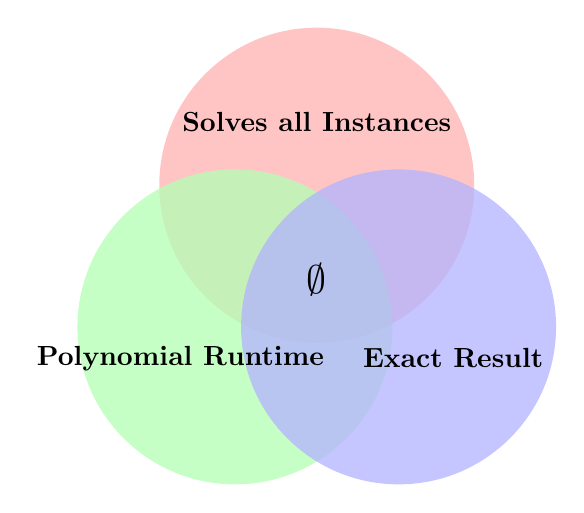
\begin{tikzpicture}
  \begin{scope}[blend mode = normal,opacity=0.75]
    \fill[red!30!white]   ( 90:1.2) circle (2);
    \fill[green!30!white] (210:1.2) circle (2);
    \fill[blue!30!white]  (330:1.2) circle (2);
  \end{scope}
  \node at ( 90:2)    {\textbf{Solves all Instances}};
  \node at ( 210:2)   {\textbf{Polynomial Runtime}};
  \node at ( 330:2)   {\textbf{Exact Result}};
  \node [font=\Large] {$\emptyset$};
\end{tikzpicture}

\end{center}
\end{frame}


\begin{frame}[c]{Ways to Cope with NP-Complete Problems}
\begin{columns}[c]
    \begin{column}{.48\textwidth}
\begin{center}
    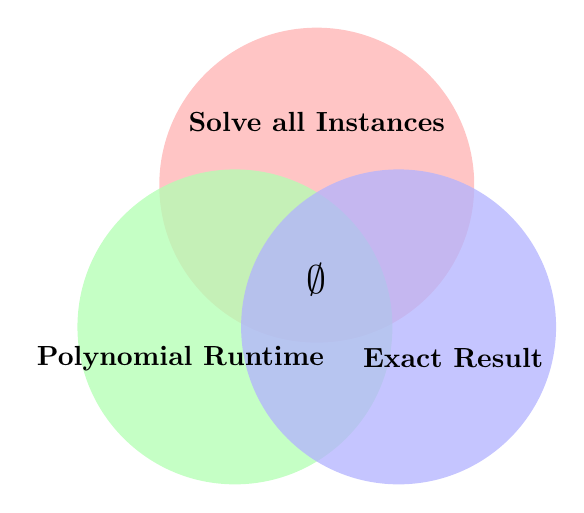
\begin{tikzpicture}
  \begin{scope}[blend mode = normal,opacity=0.75]
    \fill[red!30!white]   ( 90:1.2) circle (2);
    \fill[green!30!white] (210:1.2) circle (2);
    \fill[blue!30!white]  (330:1.2) circle (2);
  \end{scope}
  \node at ( 90:2)    {\textbf{Solve all Instances}};
  \node at ( 210:2)   {\textbf{Polynomial Runtime}};
  \node at ( 330:2)   {\textbf{Exact Result}};
  \node [font=\Large] {$\emptyset$};
\end{tikzpicture}
\end{center}
\end{column}
    \begin{column}{.48\textwidth}
    We must give up at least one:
    
    \begin{itemize}
        \pause\item \textbf{Exactness: } Approximation Algorithms
        \pause\item \textbf{Polynomial Runtime: } Exact Exponential Time Algorithms 
        \pause\item \textbf{Generality: } \textcolor{blue}{\textbf{FPT Algorithms}}
    \end{itemize}
    \end{column}
\end{columns}
\end{frame}



\begin{frame}[c]{Parametrized Complexity}
\begin{itemize}
    \item \textit{Parametrized Complexity} can be seen as a \textit{2-Dimensional} complexity analysis
    \item Looking deep into the \textit{nature of the problem} to find some hidden (in)-feasibility
    \begin{itemize}
        \item Graph of small size?
        \item Planar Graph? A Tree?
        \item Forbidden Minor?
        \item Regular? Degree-Bounded?
        \item Bipartite? Chordal?\footnote{A State-of-the-art collection: \url{https://www.graphclasses.org/}}
        \item ...
    \end{itemize}
\end{itemize}
\end{frame}

\begin{frame}[c]{The Idea Behind: \textit{Bar Fight Prevention}}

\begin{exampleblock}{The Problem}
Owning a Bar is very difficult! You already know that some people might fight so you prevent certain trouble makersfrom entering. \textbf{How many do you have to block to resolve all conflicts?}
\end{exampleblock}

\begin{center}
    \begin{tikzpicture}[>=stealth', shorten >=1pt, auto,
    node distance=1cm, scale=1, 
    transform shape, align=center, 
    state/.style={circle, draw, minimum size=1cm,thick}]
		   \node[] (D) {Daniel};
		    \node[right=of D] (G) {Gerhard};
		    \node[left=of D] (B) {Bob};
		    \node[above=of B,left=of B] (A) {Alice};
		    \node[above=of D] (E) {Erik};
		    \node[above=of E] (F) {Fedor};
		    \node[above=of D,left=of F,right=of A,left=of E,above=of A] (C) {Christos};
	    
   	    	\path (A) edge (B);
    		\path (B) edge (C);
   	    	\path (B) edge (D);
    		\path (D) edge (E);
    		\path (D) edge (G);
    		\path (G) edge (F);
    		\path (E) edge (F);
    		\path (C) edge (F);
    \end{tikzpicture}
\end{center}
\end{frame}

\begin{frame}[c]{The Idea Behind: \textit{Bar Fight Prevention}}
\begin{center}
    \begin{tikzpicture}[>=stealth', shorten >=1pt, auto,
    node distance=1cm, scale=1, 
    transform shape, align=center, 
    state/.style={circle, draw, minimum size=1cm,thick}]
		   \node[fill=lightgray] (D) {Daniel};
		    \node[right=of D] (G) {Gerhard};
		    \node[fill=lightgray,left=of D] (B) {Bob};
		    \node[above=of B,left=of B] (A) {Alice};
		    \node[above=of D] (E) {Erik};
		    \node[fill=lightgray,above=of E] (F) {Fedor};
		    \node[above=of D,left=of F,right=of A,left=of E,above=of A] (C) {Christos};
	    
   	    	\path (A) edge (B);
    		\path (B) edge (C);
   	    	\path (B) edge (D);
    		\path (D) edge (E);
    		\path (D) edge (G);
    		\path (G) edge (F);
    		\path (E) edge (F);
    		\path (C) edge (F);
    \end{tikzpicture}
    
    
\end{center}

    \pause\begin{exampleblock}{Observation}
        Removing \textit{Fedor}, \textit{Daniel} and \textit{Bob} resolves all conflicts.
    \end{exampleblock}
    \pause \textbf{Assuming 1.000 guests: $2^{1000}\approx 1.07\cdot10^{301}$}
    \textcolor{red}{\textbf{Absolutely infeasible}}
    
\end{frame}

\begin{frame}{Restricting the Problem}
    \textbf{Question: } What happens if you just have a budget of $k$-people you would like to refuse?
    \\~
    
    \begin{center}
    
    \begin{tikzpicture}[>=stealth', shorten >=1pt, auto,
    node distance=1cm, scale=1, 
    transform shape, align=center, 
    state/.style={circle, draw, minimum size=1cm,thick}]
		   \node[fill=lightgray] (D) {Daniel};
		    \node[right=of D] (G) {Gerhard};
		    \node[fill=lightgray,left=of D] (B) {Bob};
		    \node[above=of B,left=of B] (A) {Alice};
		    \node[above=of D] (E) {Erik};
		    \node[fill=lightgray,above=of E] (F) {Fedor};
		    \node[above=of D,left=of F,right=of A,left=of E,above=of A] (C) {Christos};
	    
   	    	\path (A) edge (B);
    		\path (B) edge (C);
   	    	\path (B) edge (D);
    		\path (D) edge (E);
    		\path (D) edge (G);
    		\path (G) edge (F);
    		\path (E) edge (F);
    		\path (C) edge (F);
    \end{tikzpicture}
\end{center}
    
    \\~
    \pause \textbf{Assuming 1.000 guests and $k=10$: $\binom{1000}{10}\approx2.62\cdot10^{23}$}
    \textcolor{red}{\textbf{Still pretty infeasible}}
\end{frame}

\begin{frame}{Can we do better?}

    \begin{exampleblock}{Observation}
    Someone fighting with at least $k+1$ other guests must be refused, because otherwise\textbf{all other $k+1$} guests must be refused exceeding our budget
    \end{exampleblock}
    
    \begin{center}
    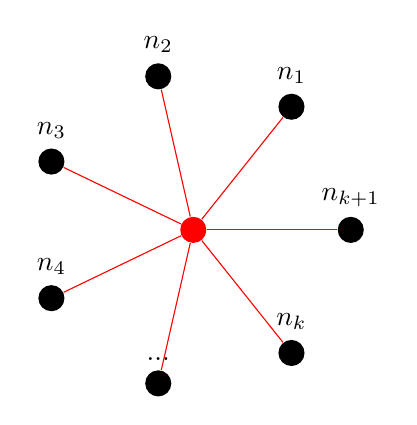
\begin{tikzpicture}
      \node[circle,fill=red] at (360:0mm) (center) {};
    \foreach \n in {1,...,4}{
        \node[circle,fill=black,label=$n_\n$] at ({\n*360/7}:2cm) (n\n) {};
        \draw[red] (center)--(n\n);
    }
        \node[circle,fill=black,label={$n_{k}$}] at ({6*360/7}:2cm) (n6) {};
        \draw[red](center)--(n6);
        \node[circle,fill=black,label={$n_{k+1}$}] at ({7*360/7}:2cm) (n7) {};
        \draw[red](center)--(n7);
        \node[circle,fill=black,label={$...$}] at ({5*360/7}:2cm) (n5) {};
        \draw[red](center)--(n5);
    \end{tikzpicture}
    \end{center}
\end{frame}

\begin{frame}[c]{Kernelization I}
\begin{itemize}
    \item $\mathtt{max}_{\mathtt{deg}} \leq k$
    \item Rejecting a guest will now resolve at most k conflicts
    \item We are allowed to remove \textbf{at most} $k$ guests each having at most $k$ conflicts
    \item If $ > k^2$ conflicts remaining: No way to resolve all: \textbf{Refuse Instance}
\end{itemize}
\begin{center}

$\binom{2k^2}{k} \leq \binom{200}{10} \approx 2.24\cdot 10^{16}$


\hbox{
\textcolor{gray}{\textbf{Feasible, but still ...}}
}
\end{center}
   \pause\textbf{Note: }This technique is called \textit{Kernelization}. 
\end{frame}

\begin{frame}[c]{Kernelization II: Improvement}

    \begin{exampleblock}{Observation}
    If $deg(n) = 1$ refuse $N[v]$ and decrease $k$ 
    \end{exampleblock}
    
\begin{columns}[T] % align columns
    \begin{column}{.48\textwidth}
 \begin{center}
    \begin{tikzpicture}
      \node[circle,fill=red,cross out=red,draw,label={$N[v]$}] at (360:0mm) (center) {};
    \foreach \n in {1,...,3}{
        \node[circle,fill=black,label=$n_\n$] at ({\n*360/4}:1.5cm) (n\n) {};
        \draw (center)--(n\n);
    }
        \node[circle,fill=orange,label={$\mathbf{v}$}] at ({4*360/4}:2cm) (n7) {};
        \draw (center)--(n7);
    \end{tikzpicture}
    \end{center}
\end{column}%
\begin{column}{.48\textwidth}
\textbf{Analysis}
\begin{itemize}
    \item Degree now bounded by $1 < \mathtt{deg}(v) <= k$
    \item $\binom{k^2}{k} \leq \binom{100}{10} \approx 1.73  \cdot 10^{13}$
    \item \textbf{Even Better!} 
\end{itemize}
\end{column}%
\end{columns}
\end{frame}

\begin{frame}{A Different Approach: Bounded Search Trees}
\begin{alertblock}{Crucial Observation}
Every conflict \textit{must} be resolved. 

$\Rightarrow$ For every conflicting pair \textbf{at least one must be refused }\footnote{This also leads to  2-approximation algorithm! (See: \cite[Ch. 35.1]{CLRS})}

\end{alertblock}

\begin{columns}[T] % align columns
    \begin{column}{.48\textwidth}
    \begin{center}
            \pause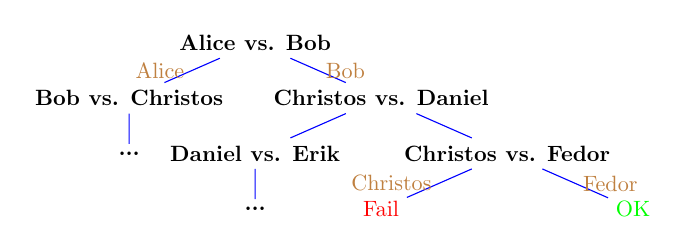
\begin{tikzpicture}[scale=0.8,transform shape]
            \node {\textbf{Alice vs. Bob}} [sibling distance = 4cm, level distance = 25pt]
                child {node {\textbf{Bob vs. Christos}}
                    child {node {\textbf{...} }}
                edge from parent [blue] node [left, brown] {Alice} 
                }
                child {node {\textbf{Christos vs. Daniel}}
                        child {node {\textbf{Daniel vs. Erik}}
                            child {node {\textbf{...}}}
                        }
                        child {node [sibling distance=1cm] {\textbf{Christos vs. Fedor}}
                                child {node {\textcolor{red}{Fail}}
                                    edge from parent [blue] node [left, brown] {Christos}
                                }
                                child {node {\textcolor{green}{OK}}
                                    edge from parent [blue] node [right, brown] {Fedor}
                                }
                        }
                edge from parent [blue] node [right, brown] {Bob}
                };
            \end{tikzpicture}
        \end{center}
    \end{column}
   \pause\begin{column}{.48\textwidth}
  \begin{center}
    \begin{tikzpicture}[>=stealth', shorten >=1pt, auto,
    node distance=1cm, scale=0.7, 
    transform shape, align=center, 
    state/.style={circle, draw, minimum size=1cm,thick}]
		   \node[fill=lightgray] (D) {Daniel};
		    \node[right=of D] (G) {Gerhard};
		    \node[fill=lightgray,left=of D] (B) {Bob};
		    \node[above=of B,left=of B] (A) {Alice};
		    \node[above=of D] (E) {Erik};
		    \node[fill=lightgray,above=of E] (F) {Fedor};
		    \node[above=of D,left=of F,right=of A,left=of E,above=of A] (C) {Christos};
	    
   	    	\path (A) edge (B);
    		\path (B) edge (C);
   	    	\path (B) edge (D);
    		\path (D) edge (E);
    		\path (D) edge (G);
    		\path (G) edge (F);
    		\path (E) edge (F);
    		\path (C) edge (F);
    \end{tikzpicture}
\end{center}
    \end{column}
\end{columns}
\end{frame}


\begin{frame}[c]{Final Runtime Using Branching}

\begin{itemize}

\item We branch into \textbf{two sub-branches} and always \textbf{decrease k by one}.
\pause \item Traversing the graph yields  $\mathcal{O}(m+n)$.
\pause \item Recall $ m \leq \frac{nk}{2}$ after our preciously discussed pre-processing procedure
\end{itemize}

\textbf{So we finally  get: }

$$ \mathcal{O}(2^k \cdot n \cdot k)$$ 

For $n = 1.000$ and $k = 10$: $2^{10} \cdot 1.000 \cdot 10 = 10.240.000$ \dSmiley

\end{frame}

\begin{frame}[c]{Parametrized Problem}
\textbf{Main Idea:} Instead of expressing the running time as a function $T(n)$ of n, we express it as a function $T(N,k)$ of the input size $n$ and \textit{some} parameter $k$ of the input.


\begin{block}{Definition 1: Parametrized Problem}
A parametrized problem is a $L\subseteq\Sigma^*\times N$ ($\Sigma$ finite fixed alphabet) for an instance $(x,k)\in \Sigma^*\times \mathrm{N}$, where k is called the \textcolor{orange}{parameter}.
\end{block}
\textbf{Examples for a parameter k:}
\begin{itemize}
    \item size k of a $\mathtt{VERTEX COVER}$
    \item size k of a $\mathtt{INDEPENDENT SET}$
    \item Treewidth k of a given graph
\end{itemize}
\end{frame}


\begin{frame}[c]{The Class FPT}

\begin{block}{Definition 2: Fixed-Parameter Tractable}
A parametrized problem $L\subseteq\Sigma^*\times\mathbb{N}$ is called \textit{fixed-parameter tractable (FPT)} if there exists an algorithm A (called a \textit{fixed-parameter algorithm}), a computable function $f:\mathbb{N} \rightarrow \mathbb{N}$ and a constant c such that, given $(x,k) \in \Sigma^* \times \mathbb{N}$, the algorithm \mathcal{A} correctly decides whether $(x,k) \in L$ in time bounded by $f(k) \cdot |(x,k)|^c$. The complexity class containing all fixed-parameter tractable problems is called \textcolor{blue}{FPT}.
\end{block}

\textbf{Note: } We often omit the polynomial-factor and rewrite the running time simply as $\mathcal{O}^*(f(k))$ 
\end{frame}

\begin{frame}[c]{The Class XP}

\begin{block}{Definition 3: Slice-Wise Polynomial}
A parametrized problem $L\subseteq \Sigma^* \times \mathbb{N}$ is called \textit{slice-wise polynomial} (XP) if there exists an algorithms \mathcal{A} and two computable functions $f,g:\mathbb{N}\rightarrow \mathbb{N}$ such that, given $(x,k) \in \Sigma^* \times \mathbb{N}$, the algorithm \mathcal{A} correctly decides whether $(x,k) \in L$ in time bounded by $f(k)\cdot|(x,k)|^{g(k)}$. The complexity class containing all slice-wise polynomial problems is called XP. 

\end{block}

\begin{alertblock}{XP vs FPT}
The class XP allows algorithms of the form $f(k) \cdot n^{g(k)}$ in contrast to FPT which tries to fix a polynomial constant c: $f(k)\cdot |(x,)|^c$. 

it can be shown: $FPT \subset XP$ by diagnolization.
\end{alertblock}
\end{frame}

\begin{frame}[c]{Vertex Cover}
\begin{itemize}
    \item The attentive listener might already have noticed that the introductory problem presented equals the NP-Complete $\mathtt{VERTEX~COVER}$ problem!
\end{itemize}

\begin{tcolorbox}[colback=green!5,colframe=green!40!black,title=$\mathtt{MIN~VERTEX~COVER}$ (\cite{Cygan2015})]
\begin{columns}[T] % align columns
    \begin{column}{.18\textwidth}
    \\~
    
    \textbf{Input:}\\
    \textbf{Question:}
    \end{column}
    \begin{column}{.78\textwidth}
    \\~
    
    Graph G and an Integer k\\
    Does there exist a set $S$ of vertices of size at most k s.t. $G - S$ is edgeless?
    \\~
    
   \textit{In other words: Is it possible to cover all edges of $G$ with at most $k$ vertices?}
    % https://www.cs.bme.hu/~dmarx/papers/marx-tractability-slides.pdf
    \end{column}
 \begin{center}
 \end{center}
 \end{columns}
\end{tcolorbox}
\end{frame}

\begin{frame}[c]{Outlook: Advanced Algorithmic Techniques}
\begin{columns}[c] % align columns
\begin{column}{.48\textwidth}
    \begin{center}
        \includegraphics[scale=0.15]{img/wordcloud.jpg}
    \end{center}
\end{column}
\begin{column}{.48\textwidth}
    \begin{itemize}
        \item There exists many techniques to deduce fast FPT algorithms.
        \item \textit{PACE} challenges competitors to solve as many very hard instances as possible: \url{https://pacechallenge.org/}
    \end{itemize}
\end{column}
\end{columns}
\end{frame}

\begin{frame}[c]{Key Takeaways I}
\begin{center}
\begin{quote}
    If there would be just three things, you should take away...
\end{quote}
\begin{itemize}
    \pause\item Problems that are only exponential in a fixed parameter k while polynomial to the input size are called \textbf{Fixed-Parameter Tractable}
    \pause\item Uses additional information or properties about a specific instance of a problem.
    \pause\item There exists many different algorithmic techniques to obtain different FPT algorithms.
\end{itemize}
\end{center}
\end{frame}